\documentclass{article}
\usepackage[utf8]{inputenc}
\usepackage{amsmath}
\usepackage[a4paper,body={140mm,250mm}]{geometry}

\usepackage{graphicx} 
\usepackage{array} 
%\usepackage{newtxtext,newtxmath}
%\usepackage[varl]{inconsolata}

\begin{document}
\begin{titlepage}
  \begin{flushleft}\scshape
    Lund University\\
    Automatic Control\\[\smallskipamount]
    FRTN70 Project in Systems, Control and Learning\\
    Spring 2021
  \end{flushleft}
  \vspace*{0pt plus 0.3fill}
  \begin{center}
    \huge \textbf{Reinforcement Learning for Double Pendulum}\\[4mm]     
    \large\textbf{Project Plan Group H}\\[5mm]
         Cem Alpturk\footnote{\texttt{ce5368al-s@student.lu.se}}\quad
         Pukashawar Pannu\footnote{\texttt{pu6218pa-s@student.lu.se}}
  \end{center}
\begin{center}
    Project Advisor: Emil Vladu
\end{center}
\vfill
\end{titlepage}        

\section{Project Purpose}
The goal of this project is to teach a model to control a double pendulum on a cart to be standing upright, in it's equilibrium point, using reinforcement learning.

\section{Equipments and Material} \label{sec:equipment}
This project does not require any physical equipment.
It will be fully simulated.

\section{Modelling and System Design}
Focus of the project is to train a controller for the dobule pendulum and not to model the actual double pendulum on a cart.

%We are proposing the code structure seen in Figure \ref{fig:uml} for our project. Considering a structure using four different packages the project can be split up and developed independently from one another. Furthermore, the packages represent the division of labour proposed in section \ref{sec:division}
%
%%\begin{figure}[b] 
%%	\centering
%% 	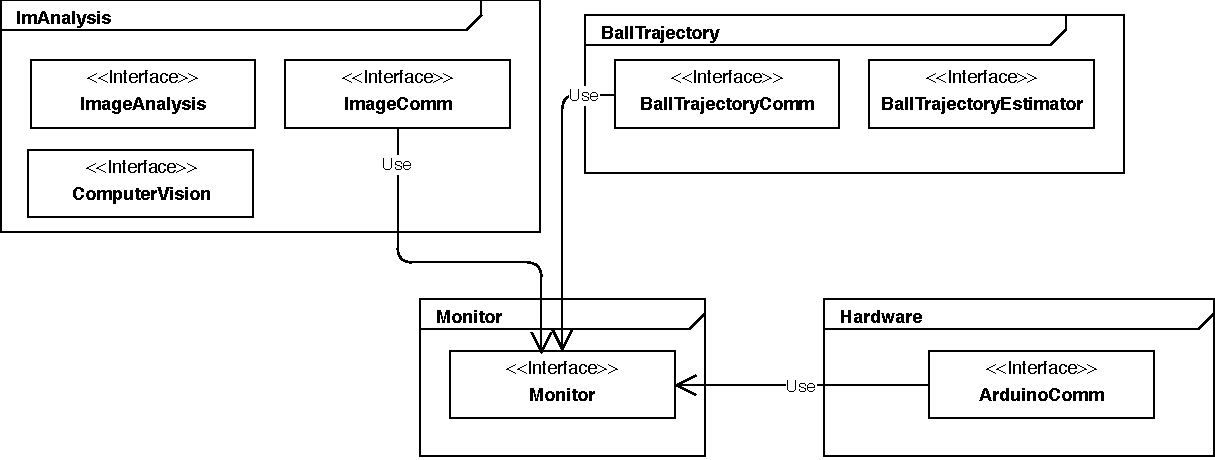
\includegraphics[width=0.85\textwidth]{figures/UML}
%%    \caption{The structure of the software.}
%%    \label{fig:uml}
%%\end{figure}
%
%\noindent
%The hardware setup will include:
%\begin{itemize}
%\item The robot arm.
%\item Two cameras mounted behind the robot.
%\item An arduino to distribute signals to the servos in the robot arm.
%\item A PC to run the software on.
%\end{itemize}
%The overall software design can be found in Figure \ref{fig:uml}. We have aimed for a design with low coupling between the different modules, the monitor package will be the central connection point of the program. This package will communicate information to the remaining packages. Since most packages will be able to run independently, they will run on different threads. Most software will be written in java, the exception being the software that will run on the arduino, this will be written in the "arduino language".


\section{Division of Labour} \label{sec:division}
We have decided to split our project into three parts: Setting up Environment, Train the Agents, Presentation. 

\subsection{Setting up Environment}
In order to teach an agent to control a double pendulum we need to simulate it.
This section is about setting up the requirements for the training phase.
Equations for the double pendulum on a cart will be researched online and from other available sources and implemented using Python.
Model will be verified by comparing with online models and an attempt will be made to animate the results to see if it looks as expected.

\subsection{Training the Agents}
This will be the main focus of the project, which is to create models and train them to control the double pendulum.
The training will utilize reinforcement learning where the agent will learn from experience by trial and error.
If the agent manages to keep the pendulum upright for a long enough time, the time has not been decided as of yet, it is considered to have solved the problem.


We have decided to split our project into three parts: image analysis, hardware and servo position implementation, and finding ball trajectory and general code structure.
	\subsection{Image analysis}
        The image analysis is a major part of our project. Without it working, we will not have a reference for the ball position. Therefore, if the image analysis is not working, we will not have a working project. We will be using two cameras (see Section \ref{sec:equipment}) to determine the position of the ball. 
    
        Olle Flitig and Sara Rask will be in charge of this section. We decided that it was a two person job since it is a quite daunting task.
    
    \subsection{Hardware and servo position}
        We will try to control the position of the servos based on a 3D point (which tells us  where the ball is supposed to land). Most of the hardware implementation and the servo control will be handled by this package. Björn Duktig is in charge of this section.
    
    \subsection{Ball trajectory and general code structure}
        We will try to estimate the final position of the ball based on a few Cartesian points (identified by the image analysis section). Furthermore, the general structure of the code will be handled by this task (e.g. the observer-observable implementation and the semaphores in the monitor). Amanda P. Solver is in charge of this section. It is also planned that she will aid in the "optimal" trajectory estimation for the robot arm (Hardware section).

\section{Time Plan}
\subsection{Subtasks}
	\begin{itemize}
		\item Search online sources for the equations of motion for the double pendulum and implement it in Python. Compare pendulum behavior to other available simulations in order to make sure that the behavior is accurate. \textbf{Estimated Deadline}: \textbf{To be decided}
		\item Animate the model using available Python libraries. \textbf{Estimated Deadline}: \textbf{To be decided}
		\item Train a model that is able to keep the pendulums in the most stable equilibrium point (down) in the presence of disturbances. \textbf{Estimated Deadline}: \textbf{To be decided}
		\item Train a model that is able to keep both pendulum in upright position without any disturbances. \textbf{Estimated Deadline}: \textbf{To be decided}
		\item Train a model that is able to keep both pendulums in upright position in the presence of disturbances. \textbf{Estimated Deadline}: \textbf{To be decided}
		\item Train a model that can transition from downright to upright position (swing-up). \textbf{Estimated Deadline}: \textbf{To be decided}
	\end{itemize}
%    \begin{itemize}
%        \item Create a Monitor package including classes used by the image analysis and the hardware systems. Implement Observer-Observable and real time behaviour. \textbf{Estimated deadline}: 31/3
%        \item Assemble the robot arm. \textbf{Estimated deadline}: 9/4
%        \item Set up a display in such a way that the cameras and the robot arm have stationary positions. \textbf{Estimated deadline}: 14/4
%        \item Implement communication between arduino and PC. \textbf{Estimated deadline}: 21/4
%        \item Find mathematical model for how the ball trajectory should be estimated. Implement this into the ballTrajectory package. \textbf{Estimated deadline}: 29/4
%        \item Find a model for the arm trajectory. \textbf{Estimated deadline}: 29/4 
%        
%        \item Create a package for how the servos should respond to the given arm trajectory. \textbf{Estimated deadline}: 6/5
%        \item Perform image segmentation to find the ball in the two cameras. \textbf{Estimated deadline}: 13/5
%        \item Make a computer vision system to map the ball segments in the images to a 3D-coordinate. Including calibration and on-line calculations. \textbf{Estimated deadline}: 13/5
%        \item (Optional); Implement feedback control of robot arm position \textbf{Estimated deadline}: N/A
%    \end{itemize}
    
\subsection{Important dates}
    \begin{itemize}
        \item Mar 29 -  Hand in project plan.
        \item Apr 22 - Feedback seminar 1 on the modeling and design.
        \item May 5 - Report should be pushed to git to allow peer review by other groups.
        \item May 11 - Peer review done
        \item May 12 - Feedback seminar 2 on the design and implementation.
        \item May 20 - Project done and demonstrated and final report handed in
        \item May 27 - Demo film upload and peer review of final report done
        \item June 3 - Final presentation and demonstration and revised final report handed in
    \end{itemize}

%\subsection{Gantt Chart}
%    We have formalized the time plan as a Gantt chart. The major tasks can be seen plotted in Figure~\ref{fig:gantt}.
%    \begin{figure}
%        \centering
%        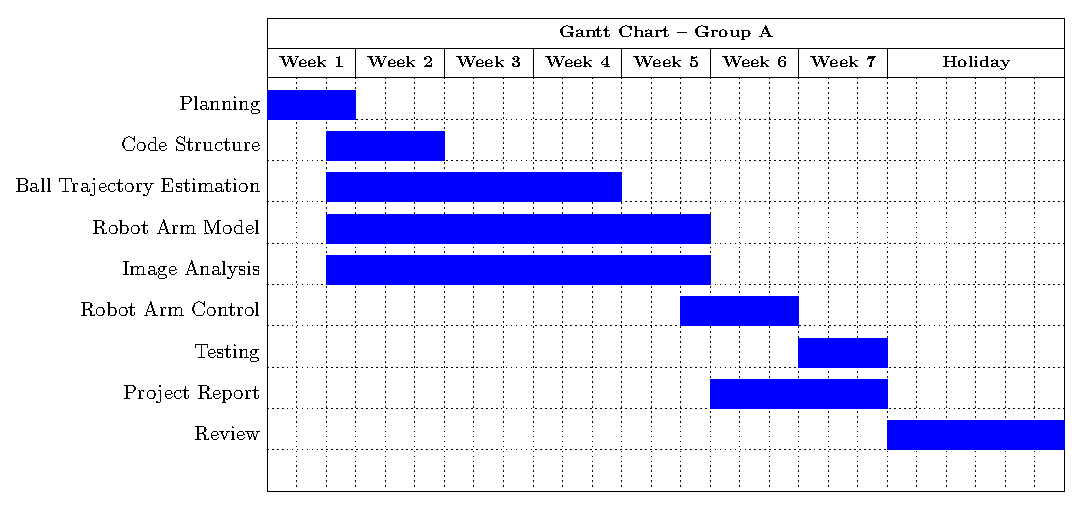
\includegraphics[width=0.95\textwidth]{figures/gantt}
%        \caption{The Gantt chart describing the work flow of our project.}
%        \label{fig:gantt}
%    \end{figure}

\end{document}
